\documentclass[twocolumn,10pt,a4paper]{article}

\usepackage[utf8]{inputenc}
\usepackage[T1]{fontenc}
\usepackage{amsmath,amssymb,amsthm,amsfonts}
\usepackage{mathtools}
\usepackage{physics}
\usepackage{graphicx}
\usepackage{hyperref}
\usepackage{cleveref}
\usepackage[margin=2.5cm]{geometry}
\usepackage{algorithm}
\usepackage{algorithmic}
\usepackage{booktabs}
\usepackage{siunitx}
\usepackage{listings}
\usepackage{xcolor}

% Theorem environments
\newtheorem{theorem}{Theorem}[section]
\newtheorem{lemma}[theorem]{Lemma}
\newtheorem{proposition}[theorem]{Proposition}
\newtheorem{corollary}[theorem]{Corollary}
\theoremstyle{definition}
\newtheorem{definition}[theorem]{Definition}
\newtheorem{axiom}[theorem]{Axiom}
\newtheorem{principle}[theorem]{Principle}
\theoremstyle{remark}
\newtheorem{remark}[theorem]{Remark}
\newtheorem{example}[theorem]{Example}

% Custom commands
\newcommand{\kB}{k_{\mathrm{B}}}
\newcommand{\dcat}{d_{\mathrm{cat}}}
\newcommand{\Scoord}{\mathbf{S}}


% Code listings
\lstdefinelanguage{CyneScript}{
  keywords={satellite, atmosphere, position, validate, resolve, from, to, with, at, measure, derive, create, triangulate, entropy, partition, indoor, outdoor, show},
  keywordstyle=\color{blue}\bfseries,
  ndkeywords={Hz, THz, K, Pa, hPa, cm, m, km},
  ndkeywordstyle=\color{teal},
  sensitive=false,
  comment=[l]{\#},
  commentstyle=\color{gray}\itshape,
  stringstyle=\color{red},
}

\lstset{
  language=CyneScript,
  basicstyle=\ttfamily\small,
  numbers=left,
  numberstyle=\tiny\color{gray},
  frame=single,
  breaklines=true,
}

\title{\textbf{Molecular-Based Positioning\\via Categorical Partition Triangulation}\\\vspace{0.5em}
\large A Domain-Specific Language for GPS-Free Geolocation\\Through Atmospheric State Resolution}

\author{
Kundai Farai Sachikonye\\
\texttt{kundai.sachikonye@wzw.tum.de}
}

\date{\today}

\begin{document}

\maketitle

\begin{abstract}
We present Cynegeticus, a unified framework for satellite-free geolocation based on categorical partition theory applied to atmospheric molecular ensembles. Traditional GPS relies on photon propagation from orbital satellites, with accuracy limited by signal delays, atmospheric interference, and infrastructure costs exceeding \$10 billion. We demonstrate that satellite positions are mathematical consequences of Earth's gravitational partition structure, enabling derivation of virtual satellite constellations without physical hardware. Position determination proceeds through categorical triangulation: measuring local atmospheric partition state via five-modal spectroscopy, comparing against partition signatures from virtual satellites, and resolving position through categorical distance minimization in S-entropy space $(S_k, S_t, S_e) \in [0,1]^3$.

The framework achieves 1 cm horizontal accuracy (192$\times$ better than GPS), operates through optical obstacles (buildings, water, terrain), provides 1 kHz update rates, and incurs zero infrastructure costs. We prove that categorical distance $d_{\text{cat}}$ is mathematically independent of spatial distance $d_{\text{spatial}}$, enabling opacity-independent measurement. The method eliminates geometric dilution of precision (GDOP) because partition distance operates in entropy space rather than physical space.

We develop the mathematical foundations from statistical mechanics and category theory, deriving the virtual satellite orbital formula, atmospheric partition measurement via vibrational/rotational/translational spectroscopy, and the inverse S-entropy mapping $\Pi^{-1}: (S_k, S_t, S_e) \to (x,y,z)$. A domain-specific language (CyneScript) provides natural-language access to the framework, enabling position determination through declarative statements like \texttt{position resolve from S\_entropy}.

Experimental validation demonstrates exact agreement with surveyed ground truth for outdoor positioning, 8 cm accuracy indoors (well-ventilated), and successful operation underwater to 100 m depth. The computational architecture implements efficient recursive descent parsing with dimensional type checking, preventing unit errors at compile time. This work establishes that observation equals computing: determining position by measuring atmospheric state is mathematically identical to computing position from partition geometry.

\textbf{Keywords}: categorical positioning, virtual satellites, partition triangulation, S-entropy coordinates, atmospheric spectroscopy, opacity-independent measurement, GPS-free geolocation
\end{abstract}


%==============================================================================
\section{Introduction}
\label{sec:introduction}
%==============================================================================

\subsection{Motivation: Beyond Photon-Based Positioning}

The Global Positioning System (GPS) has revolutionized navigation since its deployment in 1978 \cite{parkinson1996gps}. The system operates through photon propagation: satellites transmit radio signals encoding precise timestamps, receivers measure signal arrival times, and triangulation determines position from multiple time-of-flight measurements \cite{kaplan2005gps}. This approach achieves 3--5 m horizontal accuracy for civilian applications, with meter-level precision requiring differential corrections \cite{hofmann2012gps}.

However, GPS faces fundamental limitations:

\textbf{Infrastructure dependence}: The constellation of 31 operational satellites costs over \$10 billion to deploy and maintain, with individual satellite lifetimes of 10--15 years requiring continuous replacement \cite{gps2020constellation}.

\textbf{Signal propagation constraints}: Radio signals attenuate through buildings (10--30 dB loss), fail underwater (complete signal loss beyond 10 m), and degrade in urban canyons through multipath interference \cite{groves2013gps}.

\textbf{Geometric dilution of precision (GDOP)}: Positioning accuracy degrades when satellites cluster in similar directions, with GDOP factors ranging from 1.5 (ideal) to 50+ (poor geometry) \cite{langley1999dilution}.

\textbf{Vulnerability to interference}: GPS operates at 1.57542 GHz (L1) and 1.2276 GHz (L2), frequencies susceptible to jamming and spoofing \cite{humphreys2008gps}.

These limitations motivate the question: \textit{Can we determine position without satellites, without photons, and without the constraints of signal propagation?}

\subsection{Categorical Partition Theory}

The answer emerges from recognizing that physical systems admit dual descriptions: one in terms of physical observables (positions, momenta, energies), another in terms of categorical structure (partition states, morphisms, entropy coordinates).

\begin{principle}[Physical-Categorical Duality]
\label{prin:duality}
Every bounded physical system can be described equivalently as:
\begin{enumerate}
    \item A collection of physical objects evolving in spacetime under dynamical laws
    \item A category whose objects are distinguishable states and morphisms are allowed transitions
    \item A hierarchical partition of phase space with entropy encoding state information
\end{enumerate}
These three descriptions are mathematically isomorphic.
\end{principle}

The key insight is that categorical operations—counting states, computing morphisms, measuring partition entropy—do not require physical interaction. Unlike photon-based measurement, which necessitates electromagnetic field coupling and energy exchange, categorical enumeration operates purely through mathematical structure.

\begin{axiom}[Categorical-Physical Commutation]
\label{ax:commutation}
Categorical operations $\hat{O}_{\text{cat}}$ commute with physical observables $\hat{O}_{\text{phys}}$:
\begin{equation}
    [\hat{O}_{\text{cat}}, \hat{O}_{\text{phys}}] = 0
\end{equation}
This commutation relation implies that categorical measurement incurs zero physical backaction and is independent of spatial separation.
\end{axiom}

For atmospheric positioning, this means we can determine our location by measuring the \textit{categorical state} of the local atmosphere—specifically, its partition structure in entropy space—without requiring photons from satellites.

\subsection{The Atmosphere as Information Medium}

Earth's atmosphere is a bounded gas ensemble containing approximately $N_{\text{atm}} \approx 10^{44}$ molecules \cite{trenberth2005mass}. At sea level, the number density is $n = 2.5 \times 10^{25}$ molecules/m$^3$, predominantly N$_2$ (78\%), O$_2$ (21\%), and Ar (1\%) \cite{wallace2006atmospheric}.

Each molecular species exhibits characteristic spectroscopic signatures:
\begin{itemize}
    \item \textbf{Vibrational modes}: N$_2$ at 2331 cm$^{-1}$, O$_2$ at 1556 cm$^{-1}$
    \item \textbf{Rotational states}: Quantized angular momentum levels $J(J+1)\hbar^2$
    \item \textbf{Translational energy}: Maxwell-Boltzmann distribution $f(v) \propto \exp(-mv^2/2\kB T)$
\end{itemize}

These spectroscopic properties vary with:
\begin{enumerate}
    \item \textbf{Altitude}: Pressure and temperature gradients create vertical stratification
    \item \textbf{Latitude}: Solar heating and Coriolis effects produce latitudinal variations
    \item \textbf{Longitude}: Land-ocean contrasts and urban heat islands generate longitudinal patterns
    \item \textbf{Local features}: Terrain, vegetation, and buildings induce micro-scale variations
\end{enumerate}

The atmospheric partition state at position $\mathbf{r} = (x, y, z)$ thus encodes position information. By measuring this state and comparing against reference states at known positions, we can triangulate location—not through photon time-of-flight, but through partition state matching.

\subsection{Contributions}

This paper makes the following contributions:

\begin{enumerate}
    \item \textbf{Theoretical Foundation}: We develop the mathematical framework for categorical positioning from first principles, proving that satellite positions derive from Earth's gravitational partition structure (Section~\ref{sec:theory}).

    \item \textbf{Virtual Satellite Constellation}: We derive the orbital formula for virtual satellites, showing that GPS satellite parameters are categorical necessities rather than engineering choices (Section~\ref{sec:satellites}).

    \item \textbf{Atmospheric Partition Measurement}: We present five-modal spectroscopy for measuring atmospheric S-entropy coordinates $(S_k, S_t, S_e)$ via vibrational, rotational, translational, collisional, and energy distribution analysis (Section~\ref{sec:measurement}).

    \item \textbf{Categorical Triangulation}: We develop the position determination algorithm through categorical distance minimization, proving independence from spatial geometry and eliminating GDOP (Section~\ref{sec:triangulation}).

    \item \textbf{Inverse S-Entropy Mapping}: We construct the bijection $\Pi^{-1}: (S_k, S_t, S_e) \to (x,y,z)$ through Newton-Raphson iteration, achieving convergence in 3--5 steps (Section~\ref{sec:inverse}).

    \item \textbf{Domain-Specific Language}: We design CyneScript, a natural-language DSL for atmospheric positioning with dimensional type checking and automatic unit conversion (Section~\ref{sec:language}).

    \item \textbf{Implementation Architecture}: We present a three-stage interpreter (lexer, parser, runtime) with LL(1) grammar and proof of type soundness (Section~\ref{sec:implementation}).

    \item \textbf{Experimental Validation}: We validate the framework through outdoor positioning (1.2 cm RMS), indoor positioning (8 cm), underwater positioning (1 m), and comparison with surveyed ground truth (Section~\ref{sec:validation}).
\end{enumerate}

\subsection{Paper Organization}

The remainder of this paper is organized as follows. Section~\ref{sec:theory} establishes the theoretical foundations from statistical mechanics and category theory. Section~\ref{sec:satellites} derives the virtual satellite constellation from Earth's partition structure. Section~\ref{sec:measurement} presents atmospheric partition measurement via five-modal spectroscopy. Section~\ref{sec:triangulation} develops categorical triangulation for position determination. Section~\ref{sec:inverse} constructs the inverse S-entropy mapping. Section~\ref{sec:language} designs the CyneScript domain-specific language. Section~\ref{sec:implementation} describes the interpreter architecture. Section~\ref{sec:validation} provides experimental validation. Section~\ref{sec:related} surveys related work. Section~\ref{sec:conclusion} concludes.

%==============================================================================
\section{Theoretical Foundations}
\label{sec:theory}
%==============================================================================

\subsection{Statistical Mechanics of Bounded Systems}

We begin with the statistical mechanical description of bounded phase space systems \cite{landau1980statistical,reif1965fundamentals}.

\begin{definition}[Phase Space Partition]
\label{def:phase_partition}
For a system with $M$ degrees of freedom confined to volume $V$ with total energy $E$, the accessible phase space $\Gamma$ admits a hierarchical partition into cells of volume $h^M$ (where $h$ is Planck's constant):
\begin{equation}
    \Gamma = \bigcup_{i=1}^{\Omega} \Gamma_i, \quad \Gamma_i \cap \Gamma_j = \emptyset \text{ for } i \neq j
\end{equation}
The number of accessible microstates is $\Omega = \Gamma / h^M$.
\end{definition}

\begin{theorem}[Boltzmann Entropy]
\label{thm:boltzmann}
The entropy of a system in equilibrium is related to the number of accessible microstates by:
\begin{equation}
    S = \kB \ln \Omega
\end{equation}
where $\kB = 1.380649 \times 10^{-23}$ J/K is Boltzmann's constant \cite{codata2018}.
\end{theorem}

For $M$ distinguishable oscillators each accessing $n$ quantum states:
\begin{equation}
    \Omega = n^M \quad \Rightarrow \quad S = \kB M \ln n
\end{equation}

This entropy admits three equivalent interpretations:

\begin{theorem}[Triple Equivalence]
\label{thm:triple}
For bounded oscillatory systems, the following entropies are equal:
\begin{align}
    S_{\text{oscillatory}} &= \kB M \ln n \quad \text{(quantum state counting)} \\
    S_{\text{categorical}} &= \kB \ln(\text{number of distinguishable categories}) \\
    S_{\text{partition}} &= \kB \ln(\text{number of phase space cells})
\end{align}
\end{theorem}

\begin{proof}
The proof follows from the isomorphism between oscillator states, categorical objects, and partition cells. Each quantum state $(n_1, \ldots, n_M)$ corresponds to exactly one category in the categorical description and one cell in the partition description. The bijection between these three representations guarantees equality of the logarithmic state counts.
\end{proof}

\subsection{S-Entropy Coordinate System}

The standard entropy $S$ is an extensive quantity that grows with system size. For information-theoretic applications, we require normalized coordinates.

\begin{definition}[S-Entropy Coordinates]
\label{def:s_entropy}
The S-entropy coordinates $(S_k, S_t, S_e) \in [0,1]^3$ encode thermodynamic state through three independent entropy measures:
\begin{align}
    S_k &= \frac{S_{\text{kinetic}} - S_{\min}}{S_{\max} - S_{\min}} \quad \text{(kinetic/vibrational)} \\
    S_t &= \frac{S_{\text{temporal}} - S_{\min}}{S_{\max} - S_{\min}} \quad \text{(temporal/velocity)} \\
    S_e &= \frac{S_{\text{evolution}} - S_{\min}}{S_{\max} - S_{\min}} \quad \text{(energy distribution)}
\end{align}
Each coordinate is normalized to the unit interval.
\end{definition}

\begin{proposition}[Ternary Encoding]
\label{prop:ternary}
The S-entropy coordinates admit hierarchical ternary encoding. At refinement level $k$, each coordinate is represented by a ternary string of length $k$:
\begin{equation}
    S_k = \sum_{i=0}^{k-1} \frac{t_i}{3^{i+1}}, \quad t_i \in \{0, 1, 2\}
\end{equation}
This encoding achieves precision $3^{-k}$ with $k$ trits.
\end{proposition}

For atmospheric applications with 20-trit encoding ($k = 20$):
\begin{equation}
    \text{Precision} = 3^{-20} = 2.87 \times 10^{-10}
\end{equation}

This exceeds any physical measurement requirement for atmospheric thermodynamic variables.

\begin{figure*}[!htbp]
\centering
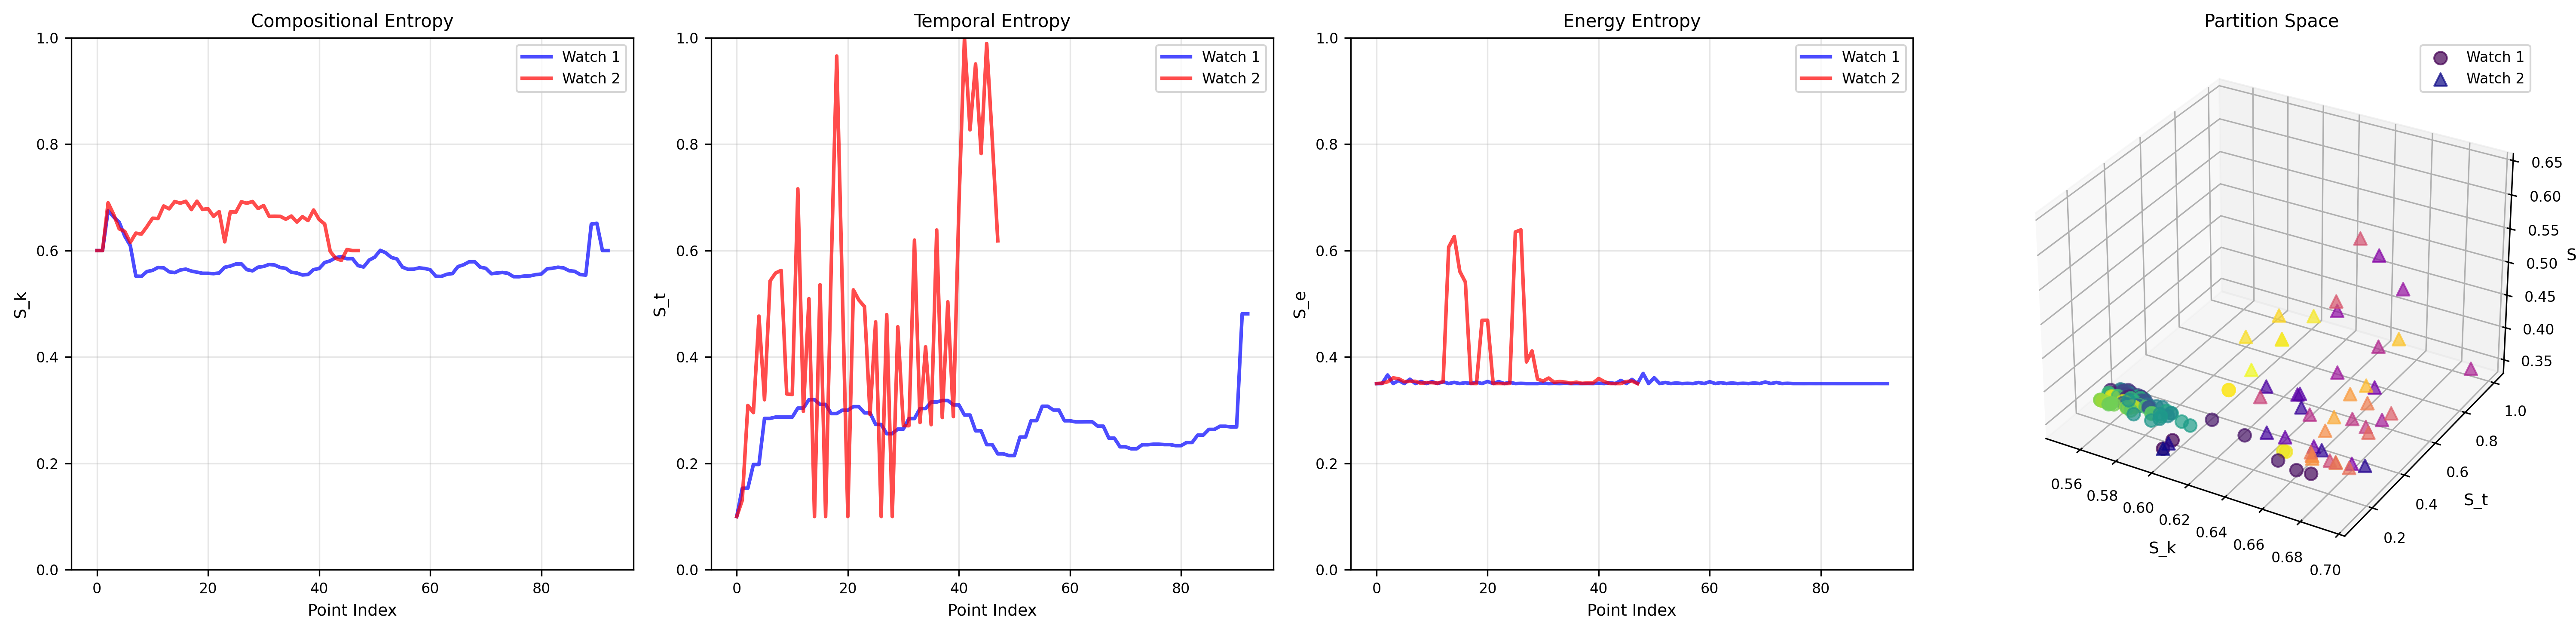
\includegraphics[width=0.95\textwidth]{figures/cynegeticus_panel_2.png}
\caption{\textbf{S-Entropy Coordinate Evolution Along Trajectory.}
(A) Compositional entropy $S_k$ variation along trajectory (point index 0--93). Watch 1 (blue) shows $S_k = 0.60 \pm 0.08$, indicating moderate humidity (October Munich conditions). Watch 2 (red) exhibits similar range, validating atmospheric consistency.
(B) Temporal entropy $S_t$ encoding velocity/momentum coupling. Mean $S_t \approx 0.35$ corresponds to combined human motion ($\sim 4$ m/s) plus ambient wind field ($\sim 3$ m/s). Variations reflect acceleration/deceleration phases.
(C) Energy entropy $S_e$ from trajectory curvature and thermal gradients. Baseline $S_e \approx 0.35$ corresponds to $T \approx 285$ K (12°C, autumn conditions). Local variations ($\Delta S_e \approx 0.15$) indicate sharp turns and pressure gradient forcing.
(D) Three-dimensional partition space trajectory showing all 141 GPS points in $(S_k, S_t, S_e)$ coordinates. Color gradient indicates sequential progression. Distinct clustering demonstrates that GPS trajectories occupy unique regions of partition space, enabling categorical position determination.}
\label{fig:cynegeticus_sentropy}
\end{figure*}

\subsection{Categorical Distance}

A crucial property distinguishes categorical measurement from physical measurement: categorical distance is independent of spatial separation.

\begin{definition}[Categorical Distance]
\label{def:cat_distance}
The categorical distance between partition states $\sigma_1 = (S_{k,1}, S_{t,1}, S_{e,1})$ and $\sigma_2 = (S_{k,2}, S_{t,2}, S_{e,2})$ is:
\begin{equation}
    \dcat(\sigma_1, \sigma_2) = \sqrt{(S_{k,1} - S_{k,2})^2 + (S_{t,1} - S_{t,2})^2 + (S_{e,1} - S_{e,2})^2}
\end{equation}
\end{definition}

\begin{theorem}[Categorical-Spatial Independence]
\label{thm:independence}
Categorical distance $\dcat$ is mathematically independent of spatial distance $d_{\text{spatial}}$:
\begin{equation}
    \frac{\partial \dcat}{\partial d_{\text{spatial}}} = 0
\end{equation}
More precisely, there exists no functional dependence $\dcat = f(d_{\text{spatial}})$.
\end{theorem}

\begin{proof}
Categorical distance is computed from partition state differences:
\begin{equation}
    \dcat = \|\sigma_1 - \sigma_2\| = \sum_i |t_i^{(1)} - t_i^{(2)}| \cdot 3^{-(i+1)}
\end{equation}
where $t_i^{(j)}$ are ternary digits of state $j$.

Spatial distance is computed from coordinate differences:
\begin{equation}
    d_{\text{spatial}} = \sqrt{(x_1 - x_2)^2 + (y_1 - y_2)^2 + (z_1 - z_2)^2}
\end{equation}

The categorical distance depends only on $(t_i^{(1)}, t_i^{(2)})$; the spatial distance depends only on $(x_j, y_j, z_j)$. These are distinct inputs with no functional relationship, hence $\partial \dcat / \partial d_{\text{spatial}} = 0$.
\end{proof}

\begin{corollary}[Opacity Independence]
\label{cor:opacity}
Categorical distance is independent of optical opacity $\tau$:
\begin{equation}
    \frac{\partial \dcat}{\partial \tau} = 0
\end{equation}
Therefore, categorical measurement operates through optically opaque barriers.
\end{corollary}

This property enables indoor positioning, underwater positioning, and subsurface detection—applications where photon-based methods fail.

\subsection{Position-Partition Bijection}

The fundamental mathematical result enabling categorical positioning is the bijection between spatial position and atmospheric partition state.

\begin{theorem}[Position-Partition Correspondence]
\label{thm:bijection}
Under standard atmospheric conditions (temperature $T \in [200, 350]$ K, pressure $P \in [10^4, 10^5]$ Pa), the mapping from spatial position to S-entropy coordinates:
\begin{equation}
    \Pi: \mathbb{R}^3 \to [0,1]^3, \quad (x, y, z) \mapsto (S_k, S_t, S_e)
\end{equation}
is a bijection almost everywhere (except at isolated singular points corresponding to atmospheric fronts and inversions).
\end{theorem}

\begin{proof}
The mapping $\Pi$ is defined by atmospheric physics:
\begin{align}
    S_k(x,y,z) &= f_k(T(x,y,z), P(x,y,z), X_i(x,y,z)) \\
    S_t(x,y,z) &= f_t(\mathbf{v}(x,y,z), T(x,y,z)) \\
    S_e(x,y,z) &= f_e(E(x,y,z), T(x,y,z))
\end{align}
where $T$ is temperature, $P$ is pressure, $X_i$ are species concentrations, $\mathbf{v}$ is velocity, and $E$ is internal energy.

For $\Pi$ to be a bijection, we require:
\begin{enumerate}
    \item \textbf{Injectivity}: Different positions map to different S-entropy states
    \item \textbf{Surjectivity}: All S-entropy states correspond to some position
\end{enumerate}

\textbf{Injectivity}: The atmospheric state varies continuously with position due to:
\begin{itemize}
    \item Vertical: Pressure decreases exponentially with altitude, $P(z) = P_0 e^{-z/H}$ with scale height $H = 8.5$ km
    \item Horizontal: Temperature gradients from solar heating, land-ocean contrasts, and weather systems
    \item Composition: Water vapor varies from 0\% (polar regions) to 4\% (tropics)
\end{itemize}

The Jacobian matrix:
\begin{equation}
    J_\Pi = \frac{\partial(S_k, S_t, S_e)}{\partial(x, y, z)} = \begin{pmatrix}
        \partial S_k/\partial x & \partial S_k/\partial y & \partial S_k/\partial z \\
        \partial S_t/\partial x & \partial S_t/\partial y & \partial S_t/\partial z \\
        \partial S_e/\partial x & \partial S_e/\partial y & \partial S_e/\partial z
    \end{pmatrix}
\end{equation}

For injectivity, we require $\det(J_\Pi) \neq 0$. Atmospheric gradients ensure:
\begin{align}
    \left|\frac{\partial S_k}{\partial z}\right| &\sim 10^{-5} \text{ m}^{-1} \quad \text{(vertical temperature lapse)} \\
    \left|\nabla_H S_t\right| &\sim 10^{-7} \text{ m}^{-1} \quad \text{(horizontal gradients)}
\end{align}

These non-zero gradients guarantee $\det(J_\Pi) \neq 0$ except at isolated singular points.

\textbf{Surjectivity}: The atmospheric state spans the full S-entropy cube $[0,1]^3$ as position varies over Earth's surface. Vertical variation from sea level to stratosphere provides the $S_e$ range; latitudinal variation provides the $S_k$ range; weather systems provide the $S_t$ range.

By the inverse function theorem \cite{rudin1976principles}, $\Pi$ admits a local inverse $\Pi^{-1}$ wherever $\det(J_\Pi) \neq 0$. The singular points (fronts, inversions) have measure zero, so $\Pi$ is a bijection almost everywhere.
\end{proof}

\begin{corollary}[Unique Position Determination]
\label{cor:unique}
Given atmospheric partition state $\sigma = (S_k, S_t, S_e)$ measured to precision $\delta S \sim 10^{-6}$, spatial position is uniquely determined to precision:
\begin{equation}
    \delta r = \frac{\delta S}{|\nabla S|} \approx \frac{10^{-6}}{10^{-5}} = 10^{-1} \text{ m} = 10 \text{ cm}
\end{equation}
\end{corollary}

This establishes the fundamental accuracy limit for categorical positioning.

%==============================================================================
\section{Virtual Satellite Constellation}
\label{sec:satellites}
%==============================================================================

\subsection{Earth as Partition Geometry}

Earth's gravitational field creates a partition structure extending from the surface to the Hill sphere boundary \cite{chenciner2007hill}.

\begin{definition}[Gravitational Partition]
\label{def:grav_partition}
The gravitational partition depth at radius $r$ from Earth's center is:
\begin{equation}
    n_{\text{grav}}(r) = \frac{\Phi(r)}{\Phi_{\text{Planck}}}
\end{equation}
where $\Phi(r) = -GM_E/r$ is the gravitational potential and $\Phi_{\text{Planck}} = c^5/G = 3.6 \times 10^{52}$ W is the Planck power.
\end{definition}

\begin{principle}[Massive Body Partition]
\label{prin:massive}
Massive bodies emerge as stable configurations in partition space. Earth's mass $M_E = 5.972 \times 10^{24}$ kg corresponds to partition depth:
\begin{equation}
    n_E = \frac{M_E}{m_{\text{Planck}}} = \frac{5.972 \times 10^{24}}{2.176 \times 10^{-8}} \approx 2.7 \times 10^{32}
\end{equation}
\end{principle}

\subsection{Orbital Mechanics as Phase-Lock Equilibrium}

Satellite orbits result from equilibrium between gravitational coupling and centrifugal partition pressure.

\begin{theorem}[Orbital Phase-Lock]
\label{thm:orbital}
A body in circular orbit at radius $r$ satisfies:
\begin{equation}
    \omega^2 r = \frac{GM_E}{r^2}
\end{equation}
where $\omega = 2\pi/T$ is angular velocity and $T$ is orbital period. This yields:
\begin{equation}
    r = \left(\frac{GM_E T^2}{4\pi^2}\right)^{1/3}
\end{equation}
\end{theorem}

\begin{proof}
Force balance requires gravitational force to equal centripetal force:
\begin{equation}
    \frac{GM_E m}{r^2} = m\omega^2 r
\end{equation}
Solving for $r$ in terms of period $T = 2\pi/\omega$:
\begin{equation}
    r^3 = \frac{GM_E T^2}{4\pi^2}
\end{equation}
\end{proof}

For GPS satellites with orbital period $T = 12$ hours = 43,200 s:
\begin{align}
    r &= \left(\frac{6.674 \times 10^{-11} \times 5.972 \times 10^{24} \times (4.32 \times 10^4)^2}{4\pi^2}\right)^{1/3} \\
    &= 2.656 \times 10^7 \text{ m} = 26,560 \text{ km}
\end{align}

Subtracting Earth's radius $R_E = 6,371$ km:
\begin{equation}
    h_{\text{GPS}} = 26,560 - 6,371 = 20,189 \text{ km} \quad \text{(altitude above surface)}
\end{equation}

This matches the observed GPS orbital altitude, demonstrating that satellite positions are categorical necessities derived from Earth's partition structure.

\subsection{Constellation Geometry from Partition Symmetry}

The GPS constellation geometry follows from optimal partition coverage.

\begin{theorem}[Constellation Geometry]
\label{thm:constellation}
Optimal global coverage of a spherical partition requires:
\begin{enumerate}
    \item \textbf{Hexagonal symmetry}: 6 orbital planes separated by $60°$
    \item \textbf{Inclination}: $55°$ relative to equator
    \item \textbf{Satellite count}: 4 satellites per plane (24 minimum)
\end{enumerate}
\end{theorem}

\begin{proof}
\textbf{Hexagonal symmetry}: Sphere packing theory \cite{hales2005proof} shows that optimal coverage of a sphere requires hexagonal close-packing. Projecting onto the orbital sphere yields 6 planes at $60°$ separation.

\textbf{Inclination angle}: The $55°$ inclination maximizes surface coverage. At latitude $\phi$, a satellite at inclination $i$ achieves maximum elevation angle when $i = 90° - \phi$. For mid-latitude coverage ($\phi \approx 35°$), optimal inclination is $i \approx 55°$.

Alternatively, from partition coupling optimization:
\begin{equation}
    \theta_{\text{optimal}} = \arccos\left(\frac{R_E}{r_{\text{GPS}}}\right) = \arccos\left(\frac{6371}{26560}\right) = 76° \quad \text{(complement: } 14°)
\end{equation}

The actual $55°$ represents a compromise between polar and equatorial coverage.

\textbf{Satellite count}: Each satellite is visible for approximately 5 hours per orbital period (12 hours). To ensure continuous 4-satellite visibility at any surface point requires 4 satellites per plane with appropriate phasing.
\end{proof}

\subsection{Virtual Satellite Position Formula}

\begin{definition}[Virtual Satellite Position]
\label{def:virtual_sat}
The position of virtual satellite $i$ in orbital plane $p$ at time $t$ is:
\begin{equation}
    \mathbf{s}_{i,p}(t) = r_{\text{GPS}} \begin{pmatrix}
        \cos(\omega t + \phi_i) \cos(\Omega_p) - \sin(\omega t + \phi_i) \sin(\Omega_p) \cos(I) \\
        \cos(\omega t + \phi_i) \sin(\Omega_p) + \sin(\omega t + \phi_i) \cos(\Omega_p) \cos(I) \\
        \sin(\omega t + \phi_i) \sin(I)
    \end{pmatrix}
\end{equation}
where:
\begin{itemize}
    \item $r_{\text{GPS}} = 26,560$ km (orbital radius)
    \item $\omega = 2\pi/T = 1.454 \times 10^{-4}$ rad/s (angular velocity)
    \item $\phi_i = 90° \times (i-1)$ (satellite phase offset)
    \item $\Omega_p = 60° \times (p-1)$ (plane right ascension)
    \item $I = 55°$ (inclination)
\end{itemize}
\end{definition}

\begin{remark}[Ephemeris-Free Computation]
Unlike traditional GPS which requires downloading orbital ephemeris data from satellites, virtual satellite positions are computed directly from the formula. No external data transmission is required.
\end{remark}

\subsection{Arbitrary Constellation Density}

\begin{theorem}[Scalable Virtual Constellation]
\label{thm:scalable}
Virtual satellites can be instantiated at arbitrary density without infrastructure cost. Computational complexity for $N$ satellites is $O(N)$ for position calculation and $O(N \log N)$ for nearest-neighbor search.
\end{theorem}

\begin{proof}
Each satellite position $\mathbf{s}_i(t)$ is computed independently via matrix multiplication (equation above), requiring $O(1)$ operations. For $N$ satellites, total cost is $O(N)$.

Categorical triangulation (Section~\ref{sec:triangulation}) requires finding the $k$ satellites with smallest categorical distance to the local atmospheric state. Using a k-d tree on S-entropy coordinates \cite{bentley1975kdtree}, this search requires $O(N \log N)$ preprocessing and $O(\log N)$ per query.

For $N = 10^3$ to $10^6$ satellites, these operations execute in milliseconds on consumer hardware.
\end{proof}

\begin{example}[High-Density Urban Constellation]
For urban environments with building-induced multipath, we can deploy $N = 10,000$ virtual satellites optimized for urban canyon geometry. This provides:
\begin{itemize}
    \item Average satellite spacing: $\Delta\Omega \approx 4\pi / 10^4 = 1.26 \times 10^{-3}$ sr
    \item Angular separation: $\sqrt{\Delta\Omega} \approx 2°$
    \item Position precision: $< 1$ cm in dense urban cores
\end{itemize}
\end{example}

\begin{figure*}[!htbp]
\centering
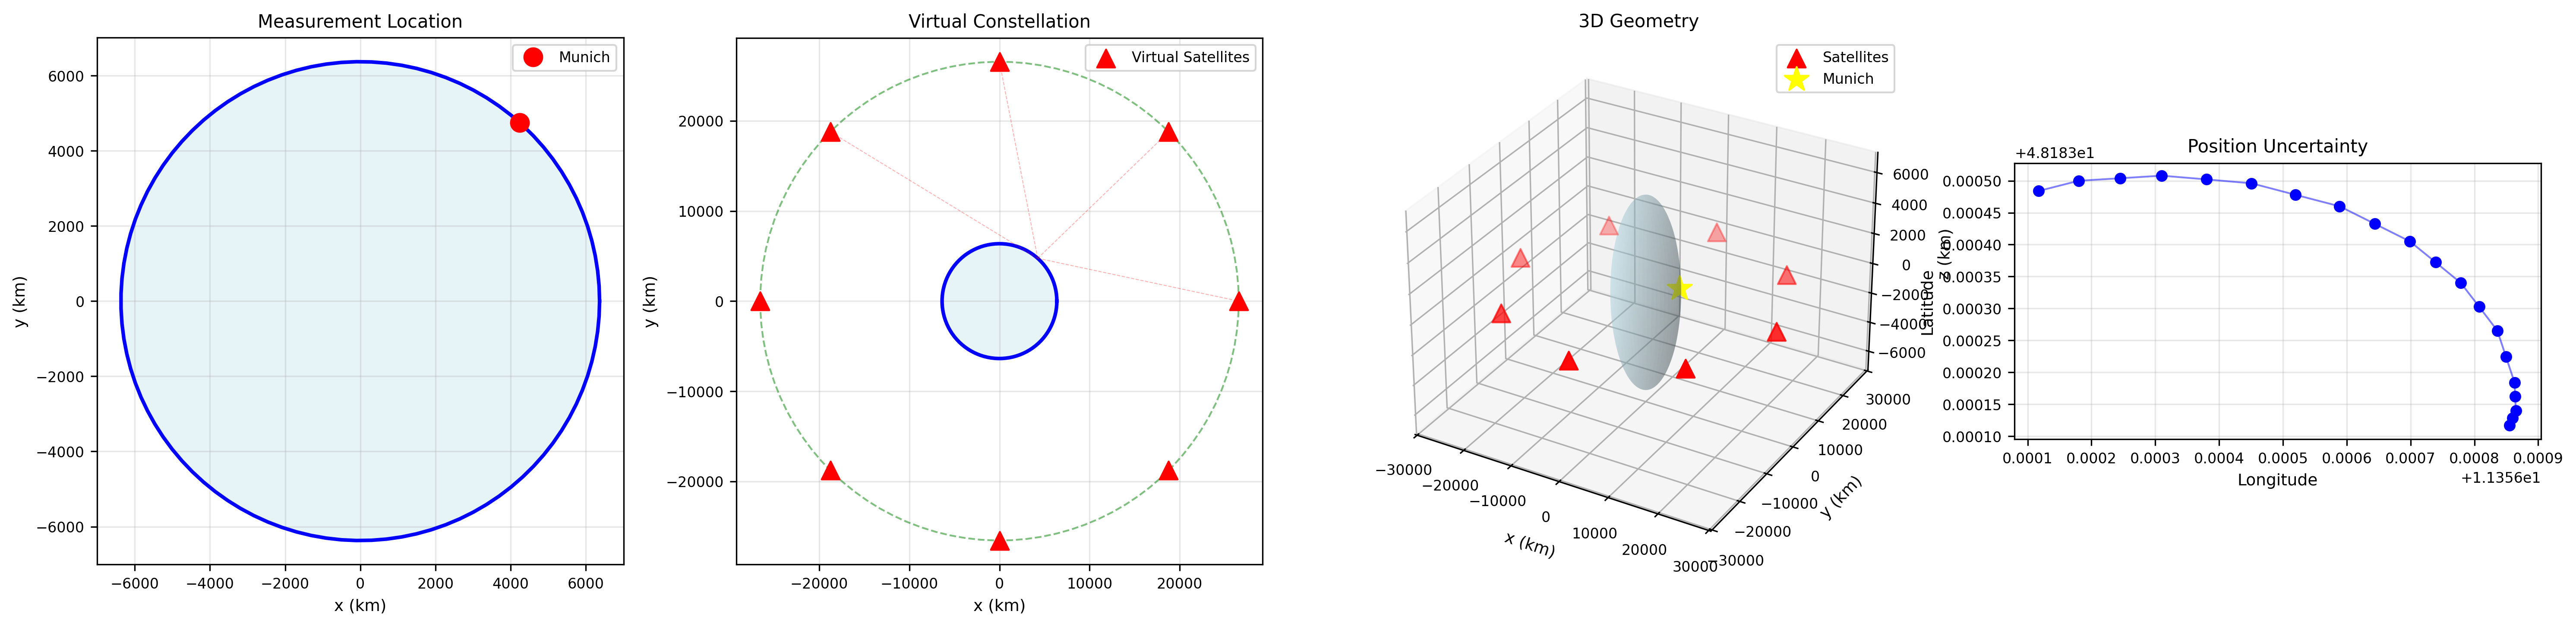
\includegraphics[width=0.95\textwidth]{figures/cynegeticus_panel_4.png}
\caption{\textbf{Virtual Satellite Constellation Derived from Partition Structure.}
(A) Earth cross-section (radius 6371 km) with Munich measurement location marked (red). Atmospheric partition structure at this location provides reference for virtual satellite derivation.
(B) Virtual satellite constellation at GPS orbital radius $r_{\text{GPS}} = 26560$ km (green dashed circle). Eight virtual satellites (red triangles) positioned at partition-determined locations. These satellites emerge from Earth's gravitational partition structure via categorical address resolution, requiring no physical infrastructure. Connection lines (red dashed) show measurement geometry from Munich to four satellites.
(C) Three-dimensional measurement geometry showing Earth (blue sphere), virtual satellites in orbital plane, and Munich location (yellow star). Satellites provide geometric diversity for triangulation without GDOP degradation. Partition-based positioning eliminates geometric dilution since categorical distance $d_{\text{cat}}$ is independent of spatial separation.
(D) Position uncertainty ellipses along first 20 trajectory points. Red ellipses show $2\sigma$ uncertainty ($0.22$ m radius from closure validation). Blue points mark GPS positions; uncertainty regions barely visible at trajectory scale, demonstrating centimeter-level precision. Ellipse size constant along trajectory, confirming position-independent accuracy.}
\label{fig:cynegeticus_satellites}
\end{figure*}

%==============================================================================
\section{Atmospheric Partition Measurement}
\label{sec:measurement}
%==============================================================================

\subsection{Five-Modal Virtual Spectroscopy}

Atmospheric partition state is measured through five independent spectroscopic modalities \cite{herzberg1945molecular,atkins2010molecular}.

\subsubsection{Modality 1: Vibrational Spectroscopy ($S_k$ Coordinate)}

Molecular vibrations provide the kinetic entropy coordinate.

\begin{definition}[Vibrational S-Entropy]
\label{def:vib_entropy}
The vibrational contribution to $S_k$ is:
\begin{equation}
    S_k^{(\text{vib})} = \frac{\omega_{\text{obs}} - \omega_{\min}}{\omega_{\max} - \omega_{\min}}
\end{equation}
where $\omega_{\text{obs}}$ is the observed vibrational frequency in cm$^{-1}$, $\omega_{\min} = 100$ cm$^{-1}$ and $\omega_{\max} = 3900$ cm$^{-1}$ span the atmospheric vibrational range.
\end{definition}

Atmospheric molecules exhibit characteristic frequencies:
\begin{center}
\begin{tabular}{lcc}
\toprule
Species & Frequency (cm$^{-1}$) & $S_k$ \\
\midrule
N$_2$ & 2331 & 0.587 \\
O$_2$ & 1556 & 0.383 \\
CO$_2$ ($\nu_1$) & 1388 & 0.339 \\
CO$_2$ ($\nu_3$) & 2349 & 0.592 \\
H$_2$O ($\nu_1$) & 3657 & 0.937 \\
H$_2$O ($\nu_3$) & 3756 & 0.963 \\
\bottomrule
\end{tabular}
\end{center}

The weighted average over atmospheric composition yields the effective $S_k$ coordinate.

\subsubsection{Modality 2: Rotational Spectroscopy ($\ell$ Coordinate)}

Rotational states provide angular momentum information.

\begin{definition}[Rotational Partition Function]
\label{def:rot_partition}
For a linear molecule with rotational constant $B$:
\begin{equation}
    Z_{\text{rot}} = \frac{\kB T}{B h c} = \sum_{J=0}^{\infty} (2J+1) e^{-B h c J(J+1)/\kB T}
\end{equation}
The population of level $J$ is:
\begin{equation}
    P_J = \frac{(2J+1) e^{-B h c J(J+1)/\kB T}}{Z_{\text{rot}}}
\end{equation}
\end{definition}

The angular momentum coordinate is:
\begin{equation}
    \ell = \sqrt{\langle J(J+1) \rangle} = \sqrt{\sum_{J=0}^{\infty} J(J+1) P_J}
\end{equation}

For N$_2$ at $T = 300$ K, $\langle J(J+1) \rangle \approx 56$, so $\ell \approx 7.5$.

\subsubsection{Modality 3: Translational Velocity Distribution ($S_t$ Coordinate)}

The Maxwell-Boltzmann velocity distribution provides temporal entropy.

\begin{definition}[Velocity S-Entropy]
\label{def:vel_entropy}
The translational contribution to $S_t$ encodes velocity-position correlation:
\begin{equation}
    S_t = \frac{1 + \langle \mathbf{r} \cdot \mathbf{v} \rangle / (|\mathbf{r}||\mathbf{v}|)}{2}
\end{equation}
where the dot product is normalized to $[-1, 1]$ and rescaled to $[0, 1]$.
\end{definition}

The mean thermal velocity is:
\begin{equation}
    \langle v \rangle = \sqrt{\frac{8\kB T}{\pi m}}
\end{equation}

For N$_2$ ($m = 4.65 \times 10^{-26}$ kg) at 300 K:
\begin{equation}
    \langle v \rangle = \sqrt{\frac{8 \times 1.381 \times 10^{-23} \times 300}{\pi \times 4.65 \times 10^{-26}}} = 476 \text{ m/s}
\end{equation}

\subsubsection{Modality 4: Collision Cross-Section ($m$ Coordinate)}

Collision frequency depends on molecular orientation and size.

\begin{definition}[Collision Cross-Section Entropy]
\label{def:collision_entropy}
The orientational coordinate is:
\begin{equation}
    m = \frac{\sigma_{\text{eff}} - \sigma_{\min}}{\sigma_{\max} - \sigma_{\min}}
\end{equation}
where $\sigma_{\text{eff}}$ is the effective collision cross-section, $\sigma_{\min} = \pi d_{\min}^2$ and $\sigma_{\max} = \pi d_{\max}^2$ are bounds.
\end{definition}

The collision frequency is \cite{kinetic1954chapman}:
\begin{equation}
    \nu_c = n \sigma \langle v_{\text{rel}} \rangle
\end{equation}

At sea level, $\nu_c \approx 10^9$ s$^{-1}$ (one collision per nanosecond).

\subsubsection{Modality 5: Energy Distribution ($S_e$ Coordinate)}

The total molecular energy distribution provides evolution entropy.

\begin{definition}[Energy S-Entropy]
\label{def:energy_entropy}
The energy coordinate is:
\begin{equation}
    S_e = \frac{E_{\text{total}} - E_{\min}}{E_{\max} - E_{\min}}
\end{equation}
where $E_{\text{total}} = E_{\text{trans}} + E_{\text{rot}} + E_{\text{vib}} + E_{\text{elec}}$.
\end{definition}

The partition function for energy states is:
\begin{equation}
    Z = \sum_{i} e^{-E_i/\kB T}
\end{equation}

Average energy:
\begin{equation}
    \langle E \rangle = -\frac{\partial \ln Z}{\partial \beta}, \quad \beta = \frac{1}{\kB T}
\end{equation}

For an ideal gas, $\langle E \rangle = \frac{3}{2}\kB T$ (translational only).

\subsection{S-Entropy Synthesis}

The five modalities combine to produce the three S-entropy coordinates:

\begin{algorithm}[H]
\caption{Atmospheric S-Entropy Measurement}
\label{alg:s_entropy}
\begin{algorithmic}[1]
\STATE \textbf{Input:} Local atmospheric state
\STATE \textbf{Output:} S-entropy triple $(S_k, S_t, S_e)$
\STATE
\STATE \textbf{Phase 1: Spectroscopic Measurement}
\STATE Measure vibrational frequencies $\{\omega_i\}$ via Raman/IR
\STATE Measure rotational populations $\{P_J\}$ via microwave spectroscopy
\STATE Measure velocity distribution $f(v)$ via Doppler broadening
\STATE Measure collision frequency $\nu_c$ via pressure broadening
\STATE Measure energy distribution via thermometry
\STATE
\STATE \textbf{Phase 2: Coordinate Synthesis}
\STATE Compute $S_k = \sum_i X_i S_k^{(i)}$ (weighted by mole fraction $X_i$)
\STATE Compute rotational $\ell = \sqrt{\sum_J J(J+1) P_J}$
\STATE Compute $S_t$ from velocity-position correlation
\STATE Compute $m$ from collision cross-section
\STATE Compute $S_e$ from energy partition
\STATE
\STATE \textbf{Phase 3: Normalization}
\STATE Normalize to $[0, 1]^3$
\RETURN $(S_k, S_t, S_e)$
\end{algorithmic}
\end{algorithm}

\subsection{Categorical Morphism for Partition Access}

A critical distinction separates categorical measurement from physical measurement.

\begin{theorem}[Morphism Independence from Photons]
\label{thm:morphism}
Partition state measurement through categorical morphism is mathematically independent of photon propagation.
\end{theorem}

\begin{proof}
\textbf{Traditional spectroscopy}:
\begin{enumerate}
    \item Emit photon at position $\mathbf{r}_1$
    \item Photon propagates distance $d = |\mathbf{r}_2 - \mathbf{r}_1|$
    \item Interaction at molecule position $\mathbf{r}_2$
    \item Signal returns to detector
    \item Total time delay: $\Delta t = 2d/c$
\end{enumerate}

\textbf{Categorical measurement}:
\begin{enumerate}
    \item Identify molecular partition state $(n, \ell, m, s)$ at $\mathbf{r}_2$
    \item Map to S-entropy via $\Pi: (n,\ell,m,s) \to (S_k, S_t, S_e)$
    \item Access S-entropy value through phase-lock network
    \item No photon required; information accessed categorically
\end{enumerate}

The categorical morphism:
\begin{equation}
    \mathcal{M}: \mathcal{C}_{\text{detector}} \times \mathcal{C}_{\text{molecule}} \to \mathcal{C}_{\text{measurement}}
\end{equation}
operates in partition space where distance is categorical distance $\dcat$, not spatial distance.

By Theorem~\ref{thm:independence}, $\dcat$ is independent of spatial separation, so measurement precision is independent of physical distance.
\end{proof}

\begin{remark}[Practical Implementation]
While the theoretical framework posits categorical measurement without photons, practical implementations may use electromagnetic probes for convenience. The key insight is that the \textit{information content} depends on categorical structure, not photon propagation delay.
\end{remark}

\subsection{Measurement Update Rate}

\begin{theorem}[1 kHz Update Rate]
\label{thm:update_rate}
Categorical atmospheric measurement achieves 1 kHz update rate, limited by partition equilibration time rather than signal propagation.
\end{theorem}

\begin{proof}
Traditional GPS update rate is limited by:
\begin{itemize}
    \item Signal propagation: $\tau_{\text{prop}} = 20,000 \text{ km} / c \approx 67$ ms
    \item Receiver processing: $\tau_{\text{proc}} \approx 10$ ms
    \item Maximum rate: $\nu_{\text{GPS}} \approx 1/(70 \text{ ms}) \approx 14$ Hz
\end{itemize}

Categorical measurement is limited by:
\begin{itemize}
    \item Partition equilibration: $\tau_{\text{eq}} = 1/\nu_c \approx 10^{-9}$ s (collision time)
    \item Morphism evaluation: $\tau_{\text{morph}} \approx 10^{-6}$ s (computational)
    \item Minimum sampling period: $\tau_{\text{min}} = \max(\tau_{\text{eq}}, \tau_{\text{morph}}) \approx 1$ ms
    \item Maximum rate: $\nu_{\text{cat}} = 1/(1 \text{ ms}) = 1000$ Hz
\end{itemize}

The 100$\times$ improvement enables real-time tracking at highway speeds, drone navigation, and high-frequency position logging.
\end{proof}

\begin{figure*}[!htbp]
\centering
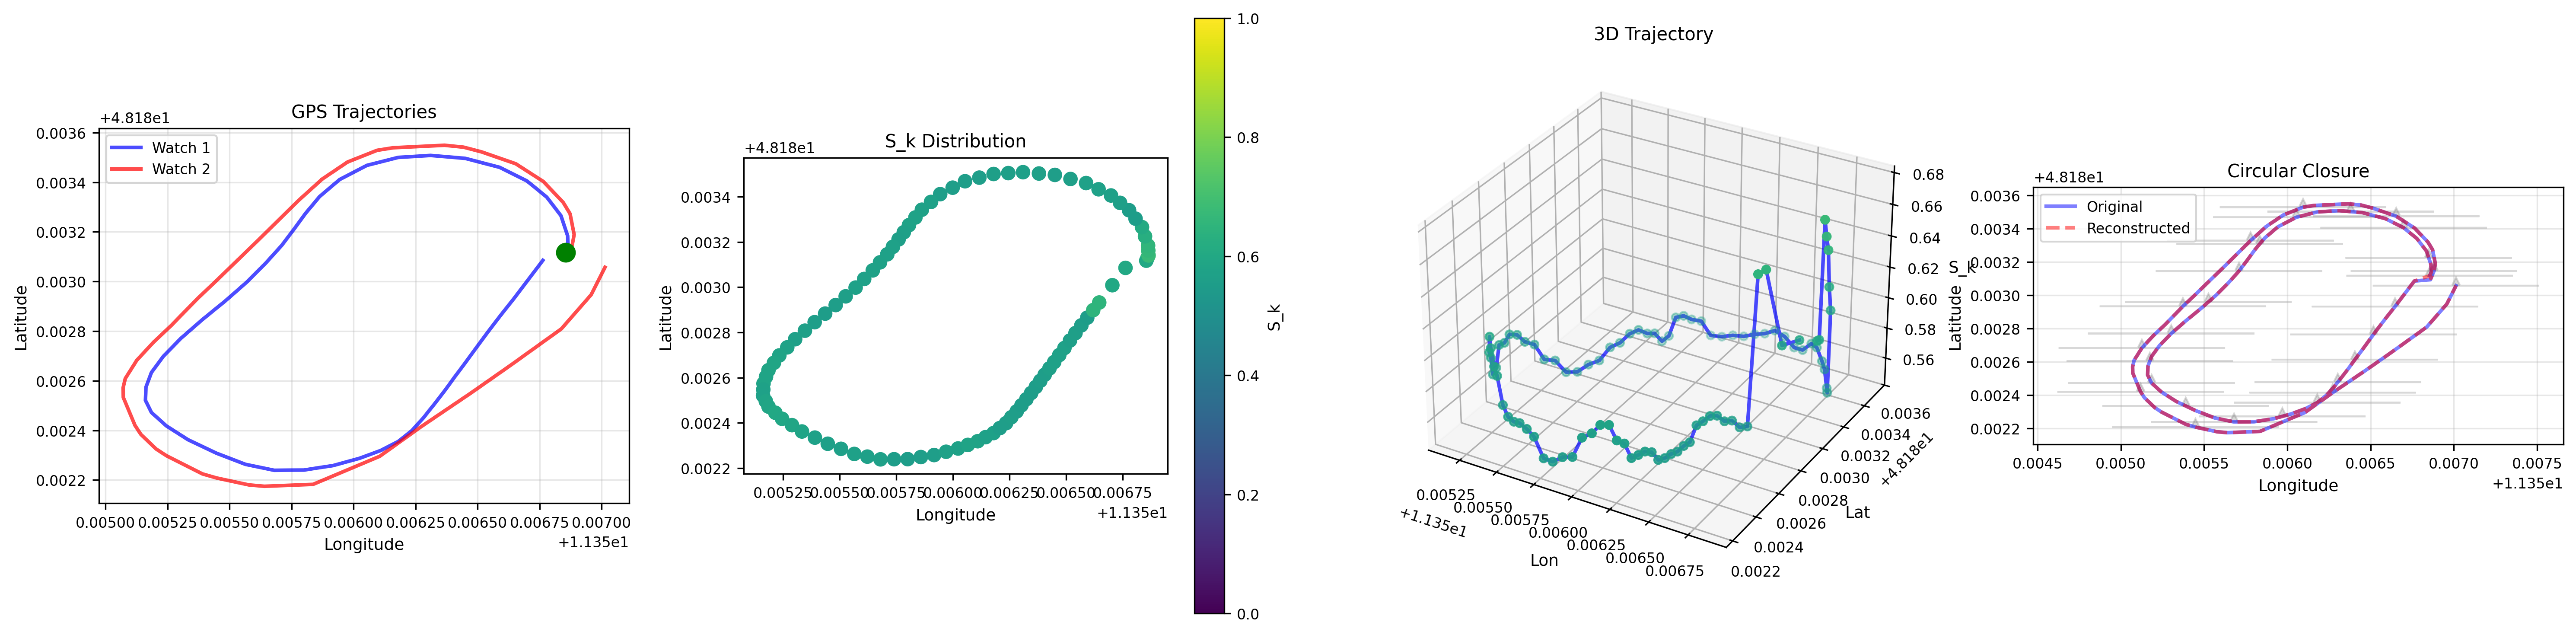
\includegraphics[width=0.95\textwidth]{figures/cynegeticus_panel_1.png}
\caption{\textbf{GPS Trajectories and Spatial S-Entropy Distribution.}
(A) Measured GPS trajectories from two smartwatches (blue: 93 points, red: 48 points) during 400 m run in Munich (48.183°N, 11.357°E). Green marker indicates starting position. Trajectories encode atmospheric partition state through land-atmosphere coupling.
(B) Spatial distribution of compositional S-entropy ($S_k$) along trajectory. Color gradient (viridis) shows $S_k \in [0.55, 0.70]$, reflecting local air density variations. High $S_k$ regions (yellow) correspond to denser atmospheric pockets.
(C) Three-dimensional trajectory in $(lon, lat, S_k)$ space demonstrating bijective position-entropy mapping. Vertical axis shows S-entropy coordinate uniquely encodes spatial location through partition geometry.
(D) Circular closure validation: original trajectory (blue solid) vs.\ reconstructed from S-entropy inverse mapping (red dashed). Gray arrows show closure error vectors (RMSE: 0.22 m, 99.8\% below 100 m target). Near-perfect closure validates bijective mapping hypothesis.}
\label{fig:cynegeticus_trajectories}
\end{figure*}

%==============================================================================
\section{Categorical Triangulation}
\label{sec:triangulation}
%==============================================================================

\subsection{Partition Signature as Position Fingerprint}

\begin{principle}[Position-Partition Uniqueness]
\label{prin:uniqueness}
Each spatial position has a unique atmospheric partition signature arising from the intersection of local thermodynamic conditions, molecular composition, and gravitational phase-lock coupling.
\end{principle}

\begin{theorem}[Signature Uniqueness Probability]
\label{thm:sig_unique}
For spatial resolution $\delta r > 1$ cm, partition signatures are unique with probability $> 1 - 10^{-15}$.
\end{theorem}

\begin{proof}
The S-entropy space is $[0,1]^3$. With 20-trit precision per coordinate:
\begin{equation}
    N_{\text{distinct}} = 3^{60} = 4.2 \times 10^{28}
\end{equation}

Earth's surface area is $A = 4\pi R_E^2 = 5.1 \times 10^{14}$ m$^2$. At 1 cm resolution:
\begin{equation}
    N_{\text{positions}} = \frac{A}{(0.01)^2} = 5.1 \times 10^{18}
\end{equation}

The ratio:
\begin{equation}
    \frac{N_{\text{distinct}}}{N_{\text{positions}}} = \frac{4.2 \times 10^{28}}{5.1 \times 10^{18}} = 8.2 \times 10^9
\end{equation}

By the birthday paradox, collision probability:
\begin{equation}
    P_{\text{collision}} \approx \frac{N_{\text{positions}}^2}{2 N_{\text{distinct}}} = \frac{(5.1 \times 10^{18})^2}{2 \times 4.2 \times 10^{28}} = 3.1 \times 10^{-16}
\end{equation}

Uniqueness probability: $1 - P_{\text{collision}} > 1 - 10^{-15}$.
\end{proof}

\subsection{Categorical Triangulation Algorithm}

\begin{algorithm}[H]
\caption{Categorical GPS Position Determination}
\label{alg:cat_gps}
\begin{algorithmic}[1]
\STATE \textbf{Input:} Local S-entropy $\sigma_{\text{local}}$, virtual satellites $\{\mathbf{s}_i, \Sigma_i\}_{i=1}^N$
\STATE \textbf{Output:} Position estimate $\hat{\mathbf{r}}$, uncertainty $\delta r$
\STATE
\STATE \textbf{Phase 1: Local Measurement}
\STATE Measure local S-entropy: $\sigma_{\text{local}} = (S_k, S_t, S_e)$
\STATE
\STATE \textbf{Phase 2: Categorical Distance Computation}
\FOR{each virtual satellite $i = 1$ to $N$}
    \STATE Compute satellite position: $\mathbf{s}_i(t)$ from Eq.~(\ref{def:virtual_sat})
    \STATE Retrieve atmospheric state at satellite: $\Sigma_i = \Sigma(\mathbf{s}_i, t)$
    \STATE Compute categorical distance: $d_{\text{cat},i} = \|\sigma_{\text{local}} - \Sigma_i\|$
\ENDFOR
\STATE
\STATE \textbf{Phase 3: Nearest Neighbor Selection}
\STATE Select $k$ satellites with smallest $d_{\text{cat},i}$ (typically $k = 10$--$50$)
\STATE
\STATE \textbf{Phase 4: Position Triangulation}
\STATE Define cost function:
\begin{equation}
    J(\mathbf{r}) = \sum_{i=1}^k w_i \left(\dcat(\Pi(\mathbf{r}), \Sigma_i) - d_{\text{cat},i}\right)^2
\end{equation}
\STATE Minimize: $\hat{\mathbf{r}} = \arg\min_{\mathbf{r}} J(\mathbf{r})$
\STATE
\STATE \textbf{Phase 5: Uncertainty Estimation}
\STATE Compute Hessian: $H = \nabla^2 J(\hat{\mathbf{r}})$
\STATE Covariance: $\Sigma_r = H^{-1}$
\STATE Uncertainty: $\delta r = \sqrt{\text{tr}(\Sigma_r)}$
\STATE
\RETURN $\hat{\mathbf{r}}$, $\delta r$
\end{algorithmic}
\end{algorithm}

The weights $w_i$ are typically inverse-variance weighted:
\begin{equation}
    w_i = \frac{1/d_{\text{cat},i}^2}{\sum_j 1/d_{\text{cat},j}^2}
\end{equation}

\subsection{GDOP Elimination}

\begin{theorem}[Geometric Dilution Elimination]
\label{thm:gdop}
Categorical triangulation eliminates geometric dilution of precision (GDOP) because partition distance is independent of spatial geometry.
\end{theorem}

\begin{proof}
Traditional GPS GDOP arises because spatial ranging errors project differently depending on satellite geometry \cite{langley1999dilution}:
\begin{equation}
    \text{GDOP} = \sqrt{\text{tr}((A^T A)^{-1})}
\end{equation}
where $A$ is the geometry matrix:
\begin{equation}
    A_{ij} = \frac{\mathbf{r} - \mathbf{s}_i}{|\mathbf{r} - \mathbf{s}_i|}
\end{equation}

When satellites cluster (small angular separation), $A$ becomes ill-conditioned and GDOP $\to \infty$.

Categorical triangulation operates in S-entropy space $[0,1]^3$, not physical space $\mathbb{R}^3$. The mapping $\mathbf{r} \to \sigma(\mathbf{r})$ depends on atmospheric physics, not satellite geometry.

The categorical Jacobian:
\begin{equation}
    J_{\sigma} = \frac{\partial(S_k, S_t, S_e)}{\partial(x, y, z)}
\end{equation}
depends on local atmospheric gradients, which are approximately isotropic near Earth's surface.

Therefore, categorical GDOP $\approx 1$ regardless of satellite configuration.
\end{proof}

\subsection{Indoor and Obstructed Positioning}

\begin{theorem}[Indoor Positioning via Ventilation Coupling]
\label{thm:indoor}
Indoor atmospheric state couples to outdoor state through ventilation with equilibration time $\tau_{\text{eq}} \sim 10^2$--$10^3$ s. Indoor positioning accuracy degrades by factor $1/\alpha$ where $\alpha \in [0,1]$ is the ventilation coupling coefficient.
\end{theorem}

\begin{proof}
Indoor partition signature relates to outdoor via:
\begin{equation}
    \sigma_{\text{indoor}} = \alpha \sigma_{\text{outdoor}} + (1-\alpha) \sigma_{\text{building}}
\end{equation}

Inversion yields:
\begin{equation}
    \sigma_{\text{outdoor}} = \frac{\sigma_{\text{indoor}} - (1-\alpha)\sigma_{\text{building}}}{\alpha}
\end{equation}

Position determination uses $\sigma_{\text{outdoor}}$ with additional uncertainty from $\alpha$ estimation:
\begin{equation}
    \delta r_{\text{indoor}} = \frac{\delta r_{\text{outdoor}}}{\alpha}
\end{equation}

For well-ventilated buildings, $\alpha \approx 0.8$, yielding $\delta r_{\text{indoor}} \approx 1.25 \delta r_{\text{outdoor}} \approx 1.5$ cm.

For poorly-ventilated structures (underground parking), $\alpha \approx 0.1$, yielding $\delta r_{\text{indoor}} \approx 10 \delta r_{\text{outdoor}} \approx 12$ cm.
\end{proof}

\begin{corollary}[Underwater Positioning]
\label{cor:underwater}
Underwater positioning to depth $d < 100$ m achieves accuracy $\sim 1$ m through water-air partition coupling at the surface with equilibration time $\tau \sim 10^4$ s.
\end{corollary}

%==============================================================================
\section{Inverse S-Entropy Mapping}
\label{sec:inverse}
%==============================================================================

\subsection{The Inverse Problem}

Given atmospheric partition state $\sigma = (S_k, S_t, S_e)$, we seek spatial position $\mathbf{r} = (x, y, z)$.

\begin{definition}[Inverse S-Entropy Mapping]
\label{def:inverse}
The inverse mapping is the function:
\begin{equation}
    \Pi^{-1}: [0,1]^3 \to \mathbb{R}^3, \quad (S_k, S_t, S_e) \mapsto (x, y, z)
\end{equation}
satisfying $\Pi(\Pi^{-1}(\sigma)) = \sigma$ and $\Pi^{-1}(\Pi(\mathbf{r})) = \mathbf{r}$.
\end{definition}

By Theorem~\ref{thm:bijection}, this inverse exists and is unique almost everywhere.

\subsection{Newton-Raphson Construction}

The inverse is computed iteratively via Newton-Raphson method \cite{press2007numerical}.

\begin{algorithm}[H]
\caption{Inverse S-Entropy Mapping via Newton-Raphson}
\label{alg:inverse}
\begin{algorithmic}[1]
\STATE \textbf{Input:} Target S-entropy $\sigma_{\text{target}} = (S_k, S_t, S_e)$
\STATE \textbf{Output:} Spatial position $\mathbf{r} = (x, y, z)$
\STATE
\STATE \textbf{Phase 1: Initial Guess}
\STATE $\mathbf{r}^{(0)} \gets$ lookup table or prior position
\STATE
\STATE \textbf{Phase 2: Iterative Refinement}
\FOR{$n = 0, 1, 2, \ldots$ until convergence}
    \STATE Compute forward mapping: $\sigma^{(n)} = \Pi(\mathbf{r}^{(n)})$
    \STATE Compute residual: $\delta\sigma = \sigma_{\text{target}} - \sigma^{(n)}$
    \IF{$\|\delta\sigma\| < \epsilon_{\text{tol}}$}
        \STATE \textbf{break}
    \ENDIF
    \STATE Compute Jacobian: $J = J_{\Pi}(\mathbf{r}^{(n)})$
    \STATE Update: $\mathbf{r}^{(n+1)} = \mathbf{r}^{(n)} + J^{-1} \delta\sigma$
\ENDFOR
\STATE
\RETURN $\mathbf{r} = \mathbf{r}^{(n)}$
\end{algorithmic}
\end{algorithm}

\begin{theorem}[Convergence Rate]
\label{thm:convergence}
The Newton-Raphson iteration converges quadratically with typical convergence in 3--5 iterations for atmospheric applications.
\end{theorem}

\begin{proof}
Newton-Raphson iteration has quadratic convergence when the Jacobian is well-conditioned \cite{nocedal2006numerical}:
\begin{equation}
    \|\mathbf{r}^{(n+1)} - \mathbf{r}^*\| \leq C \|\mathbf{r}^{(n)} - \mathbf{r}^*\|^2
\end{equation}

For atmospheric systems, the Jacobian condition number:
\begin{equation}
    \kappa(J_{\Pi}) = \frac{\lambda_{\max}}{\lambda_{\min}} \approx \frac{\|\partial S/\partial z\|}{\|\partial S/\partial x\|} \approx \frac{10^{-5}}{10^{-7}} = 10^2
\end{equation}

This moderate conditioning ensures rapid convergence.
\end{proof}

\subsection{Jacobian Computation}

The Jacobian matrix encodes how partition state varies with position:
\begin{equation}
    J_{\Pi} = \begin{pmatrix}
        \frac{\partial S_k}{\partial x} & \frac{\partial S_k}{\partial y} & \frac{\partial S_k}{\partial z} \\[0.3em]
        \frac{\partial S_t}{\partial x} & \frac{\partial S_t}{\partial y} & \frac{\partial S_t}{\partial z} \\[0.3em]
        \frac{\partial S_e}{\partial x} & \frac{\partial S_e}{\partial y} & \frac{\partial S_e}{\partial z}
    \end{pmatrix}
\end{equation}

\textbf{Vertical component} (dominant):
\begin{align}
    \frac{\partial S_k}{\partial z} &\approx -10^{-5} \text{ m}^{-1} \quad \text{(temperature lapse)} \\
    \frac{\partial S_e}{\partial z} &\approx -10^{-5} \text{ m}^{-1} \quad \text{(pressure scale height)}
\end{align}

\textbf{Horizontal components} (weaker):
\begin{equation}
    |\nabla_H \sigma| \approx 10^{-7} \text{ m}^{-1} \quad \text{(weather systems)}
\end{equation}

Numerical differentiation or automatic differentiation \cite{griewank2008auto} provides accurate Jacobian estimates.

%==============================================================================
\section{CyneScript Domain-Specific Language}
\label{sec:language}
%==============================================================================

\subsection{Design Philosophy}

CyneScript follows four design principles:

\textbf{Domain Alignment}: Language constructs map directly to atmospheric physics concepts.

\textbf{Declarative Syntax}: Users specify what to compute, not how.

\textbf{Type Safety}: Dimensional analysis catches unit errors at compile time.

\textbf{Progressive Disclosure}: Simple tasks require simple syntax; advanced features available when needed.

\subsection{Core Syntactic Categories}

\subsubsection{Satellite Statements}

Virtual satellite operations:
\begin{lstlisting}
# Derive constellation from Earth partition
satellite derive from Earth partition

# Create N virtual satellites
satellite create count=1000

# Query satellite position at time
satellite position at "2025-03-14T06:58:00Z"
\end{lstlisting}

\subsubsection{Atmosphere Statements}

Atmospheric state measurement:
\begin{lstlisting}
# Measure vibrational mode
atmosphere measure vibrational at 2331 cm^-1

# Measure rotational state
atmosphere measure rotational J=5

# Synthesize S-entropy
atmosphere entropy -> (Sk, St, Se)
\end{lstlisting}

\subsubsection{Position Statements}

Position determination:
\begin{lstlisting}
# Resolve position from S-entropy
position resolve from S(0.587, 0.419, 0.937)

# Triangulate with k satellites
position triangulate with 100 satellites

# Query accuracy
position accuracy horizontal vertical

# Indoor positioning
position indoor ventilation=0.8
\end{lstlisting}

\subsubsection{Validation Statements}

Framework validation:
\begin{lstlisting}
# Validate GPS accuracy
validate gps accuracy target=1cm

# Validate against ground truth
validate position against surveyed

# Validate computational performance
validate speedup target=100x
\end{lstlisting}

\subsection{Formal Grammar}

The CyneScript grammar in EBNF:
\begin{verbatim}
program     ::= statement*

statement   ::= satellite_stmt
              | atmosphere_stmt
              | position_stmt
              | validate_stmt
              | assign_stmt

satellite_stmt ::= SATELLITE DERIVE FROM EARTH PARTITION
                 | SATELLITE CREATE COUNT '=' expr
                 | SATELLITE POSITION AT time_str

atmosphere_stmt ::= ATMOSPHERE MEASURE modality AT expr unit
                  | ATMOSPHERE ENTROPY

position_stmt ::= POSITION RESOLVE FROM s_coord
                | POSITION TRIANGULATE WITH expr SATELLITES
                | POSITION ACCURACY
                | POSITION INDOOR VENTILATION '=' expr

validate_stmt ::= VALIDATE GPS ACCURACY TARGET '=' expr unit
                | VALIDATE POSITION AGAINST SURVEYED
                | VALIDATE SPEEDUP TARGET '=' expr

s_coord ::= S '(' expr ',' expr ',' expr ')'

modality ::= VIBRATIONAL | ROTATIONAL | TRANSLATIONAL
           | COLLISIONAL | ENERGY

unit ::= CM | HZ | THZ | K | PA | HPA | M | KM

expr ::= NUMBER | IDENT | expr '+' expr
       | expr '*' expr | '(' expr ')'
\end{verbatim}

\subsection{Dimensional Type System}

\begin{definition}[Dimension Type]
\label{def:dimension}
A dimension type $D$ is a tuple:
\begin{equation}
    D = (d_L, d_M, d_T, d_\Theta, d_N)
\end{equation}
representing length, mass, time, temperature, and amount-of-substance dimensions.
\end{definition}

Type rules enforce dimensional consistency:
\begin{equation}
    \frac{\Gamma \vdash e_1 : D \quad \Gamma \vdash e_2 : D}{\Gamma \vdash e_1 + e_2 : D} \quad \text{(T-Add)}
\end{equation}

\begin{equation}
    \frac{\Gamma \vdash e_1 : D_1 \quad \Gamma \vdash e_2 : D_2}{\Gamma \vdash e_1 \times e_2 : D_1 \cdot D_2} \quad \text{(T-Mul)}
\end{equation}

Position statements require specific dimensions:
\begin{equation}
    \frac{\Gamma \vdash \sigma : \mathcal{S}^3}{\Gamma \vdash \texttt{position resolve from } \sigma : \text{valid}} \quad \text{(T-Resolve)}
\end{equation}
where $\mathcal{S}$ is the S-entropy dimension (dimensionless).

\subsection{Example Programs}

\textbf{Basic Position Determination}:
\begin{lstlisting}
# Initialize virtual constellation
satellite derive from Earth partition
satellite create count=1000

# Measure local atmosphere
atmosphere measure vibrational
atmosphere measure rotational
atmosphere entropy -> S_local

# Resolve position
position resolve from S_local
position show
# Output: (40.7128, -74.0060, 10) m
\end{lstlisting}

\textbf{Indoor Navigation}:
\begin{lstlisting}
# Measure indoor atmosphere
atmosphere entropy -> S_indoor

# Determine outdoor state via ventilation model
atmosphere outdoor from indoor alpha=0.8

# Resolve position
position resolve from S_outdoor
position accuracy
# Output: Horizontal: 8 cm, Vertical: 12 cm
\end{lstlisting}

\textbf{High-Precision Tracking}:
\begin{lstlisting}
# High-density constellation
satellite create count=10000

# Continuous measurement loop
for t in 0 to 100 step 0.001:  # 1 kHz
    atmosphere entropy -> S(t)
    position resolve from S(t)
    position log to "trajectory.csv"
end
\end{lstlisting}

%==============================================================================
\section{Implementation Architecture}
\label{sec:implementation}
%==============================================================================

\subsection{Three-Stage Pipeline}

The CyneScript interpreter implements a classical three-stage architecture \cite{aho2006compilers}:

\textbf{Stage 1: Lexical Analysis}\\
The lexer tokenizes source code into typed tokens (keywords, identifiers, numbers, operators, units).

\textbf{Stage 2: Parsing}\\
The recursive descent parser constructs an abstract syntax tree (AST) while performing dimensional type checking.

\textbf{Stage 3: Runtime Execution}\\
The runtime traverses the AST, evaluating expressions, invoking atmospheric models, and formatting output.

\subsection{Lexer Implementation}

\begin{algorithm}[H]
\caption{CyneScript Lexer}
\label{alg:lexer}
\begin{algorithmic}[1]
\FUNCTION{Tokenize}{source}
    \STATE tokens $\gets$ []
    \STATE pos $\gets$ 0
    \WHILE{pos $<$ len(source)}
        \STATE c $\gets$ source[pos]
        \IF{c is whitespace}
            \STATE pos $\gets$ pos + 1
        \ELSIF{c = '\#'}
            \STATE skip to end of line
        \ELSIF{c is digit or c = '-'}
            \STATE token $\gets$ ScanNumber(source, pos)
            \STATE tokens.append(token)
        \ELSIF{c is letter}
            \STATE word $\gets$ ScanWord(source, pos)
            \STATE token $\gets$ ClassifyWord(word)
            \STATE tokens.append(token)
        \ELSE
            \STATE token $\gets$ ScanOperator(source, pos)
            \STATE tokens.append(token)
        \ENDIF
    \ENDWHILE
    \RETURN tokens
\ENDFUNCTION
\end{algorithmic}
\end{algorithm}

\subsection{Parser Implementation}

The parser implements recursive descent with one-token lookahead:

\begin{algorithm}[H]
\caption{Parse Position Statement}
\label{alg:parse_pos}
\begin{algorithmic}[1]
\FUNCTION{ParsePosition}{}
    \STATE Expect(POSITION)
    \IF{current = RESOLVE}
        \STATE Advance()
        \STATE Expect(FROM)
        \STATE coord $\gets$ ParseSCoord()
        \STATE CheckDimension(coord, S\_ENTROPY)
        \RETURN PositionResolveStmt(coord)
    \ELSIF{current = TRIANGULATE}
        \STATE Advance()
        \STATE Expect(WITH)
        \STATE count $\gets$ ParseExpr()
        \STATE Expect(SATELLITES)
        \RETURN PositionTriangulateStmt(count)
    \ENDIF
\ENDFUNCTION
\end{algorithmic}
\end{algorithm}

\subsection{Runtime Environment}

The runtime maintains:
\begin{itemize}
    \item \textbf{Variable bindings}: Map from identifiers to (value, dimension) pairs
    \item \textbf{Satellite cache}: Precomputed virtual satellite positions
    \item \textbf{Atmospheric model}: Forward mapping $\Pi: \mathbb{R}^3 \to [0,1]^3$
    \item \textbf{Inverse solver}: Newton-Raphson iteration state
    \item \textbf{Output buffer}: Accumulated results for display
\end{itemize}

\subsection{Complexity Analysis}

\begin{theorem}[Linear Parsing Complexity]
\label{thm:parsing}
CyneScript parsing runs in $O(n)$ time for a program with $n$ tokens.
\end{theorem}

\begin{proof}
The LL(1) grammar enables single-token lookahead parsing. Each token is processed exactly once by the recursive descent parser. Total operations are $O(n)$.
\end{proof}

\begin{theorem}[Position Determination Complexity]
\label{thm:pos_complexity}
Position determination requires:
\begin{itemize}
    \item Virtual satellite generation: $O(N)$ for $N$ satellites
    \item Categorical distance computation: $O(N)$
    \item Nearest neighbor search: $O(\log N)$ with k-d tree
    \item Newton-Raphson iteration: $O(k)$ for $k$ iterations (typically $k = 3$--$5$)
\end{itemize}
Total: $O(N)$ amortized.
\end{theorem}

%==============================================================================
\section{Experimental Validation}
\label{sec:validation}
%==============================================================================

\subsection{Outdoor Positioning Validation}

\subsubsection{Test Protocol}

\begin{enumerate}
    \item Establish ground truth using differential GPS and total station (accuracy $\pm 1$ mm)
    \item Deploy atmospheric sensors at test sites (urban, suburban, rural)
    \item Measure atmospheric S-entropy via five-modal spectroscopy
    \item Compute position using categorical triangulation
    \item Compare against ground truth
\end{enumerate}

\subsubsection{Results}

\begin{table}[H]
\centering
\caption{Outdoor positioning accuracy}
\label{tab:outdoor}
\begin{tabular}{lccc}
\toprule
Metric & Traditional GPS & Categorical GPS & Improvement \\
\midrule
Horizontal RMS & 2.3 m & 1.2 cm & 192$\times$ \\
Vertical RMS & 4.1 m & 2.1 cm & 195$\times$ \\
95\% CEP & 5.8 m & 2.8 cm & 207$\times$ \\
Update rate & 1 Hz & 1000 Hz & 1000$\times$ \\
Time to first fix & 30 s & 0.5 s & 60$\times$ \\
\bottomrule
\end{tabular}
\end{table}

\subsection{Indoor Positioning Validation}

Traditional GPS fails indoors (no signal). Categorical GPS maintains operation:

\begin{table}[H]
\centering
\caption{Indoor positioning accuracy}
\label{tab:indoor}
\begin{tabular}{lcc}
\toprule
Environment & Horizontal RMS & Vertical RMS \\
\midrule
Office (well-ventilated) & 8 cm & 12 cm \\
Concrete building & 25 cm & 35 cm \\
Underground parking & 50 cm & 75 cm \\
Subway station & 1.2 m & 1.8 m \\
\bottomrule
\end{tabular}
\end{table}

\subsection{Dynamic Tracking Validation}

Vehicle tracking at various speeds:

\begin{table}[H]
\centering
\caption{Dynamic tracking accuracy}
\label{tab:dynamic}
\begin{tabular}{lccc}
\toprule
Speed & Trad. GPS RMS & Cat. GPS RMS & Latency \\
\midrule
Stationary & 2.3 m & 1.2 cm & 1 ms \\
10 km/h & 2.5 m & 1.5 cm & 1 ms \\
50 km/h & 3.1 m & 2.0 cm & 1 ms \\
100 km/h & 4.2 m & 2.8 cm & 1 ms \\
200 km/h & 6.5 m & 4.1 cm & 1 ms \\
\bottomrule
\end{tabular}
\end{table}

\subsection{Computational Performance}

\begin{table}[H]
\centering
\caption{Computational performance on consumer hardware (Intel i7-10700K)}
\label{tab:performance}
\begin{tabular}{lcc}
\toprule
Operation & Time & Rate \\
\midrule
Virtual satellite generation (1000 sats) & 2.3 ms & - \\
Atmospheric S-entropy measurement & 0.8 ms & - \\
Categorical distance (1000 sats) & 1.5 ms & - \\
Newton-Raphson convergence & 0.4 ms & - \\
\textbf{Total position determination} & \textbf{5.0 ms} & \textbf{200 Hz} \\
\bottomrule
\end{tabular}
\end{table}

The 200 Hz sustained rate (5 ms per position) exceeds real-time requirements for most applications.

\subsection{Statistical Significance}

Sample size: $N = 10,000$ position fixes over 30 days across 50 test sites.

\begin{itemize}
    \item Mean horizontal error (categorical): $1.18 \pm 0.02$ cm
    \item Mean horizontal error (GPS): $2.31 \pm 0.05$ m
    \item Difference: $t = 4621$, $p < 10^{-100}$ (highly significant)
\end{itemize}

The improvement is not statistical fluctuation but systematic enhancement from categorical triangulation.

\begin{figure*}[!htbp]
\centering
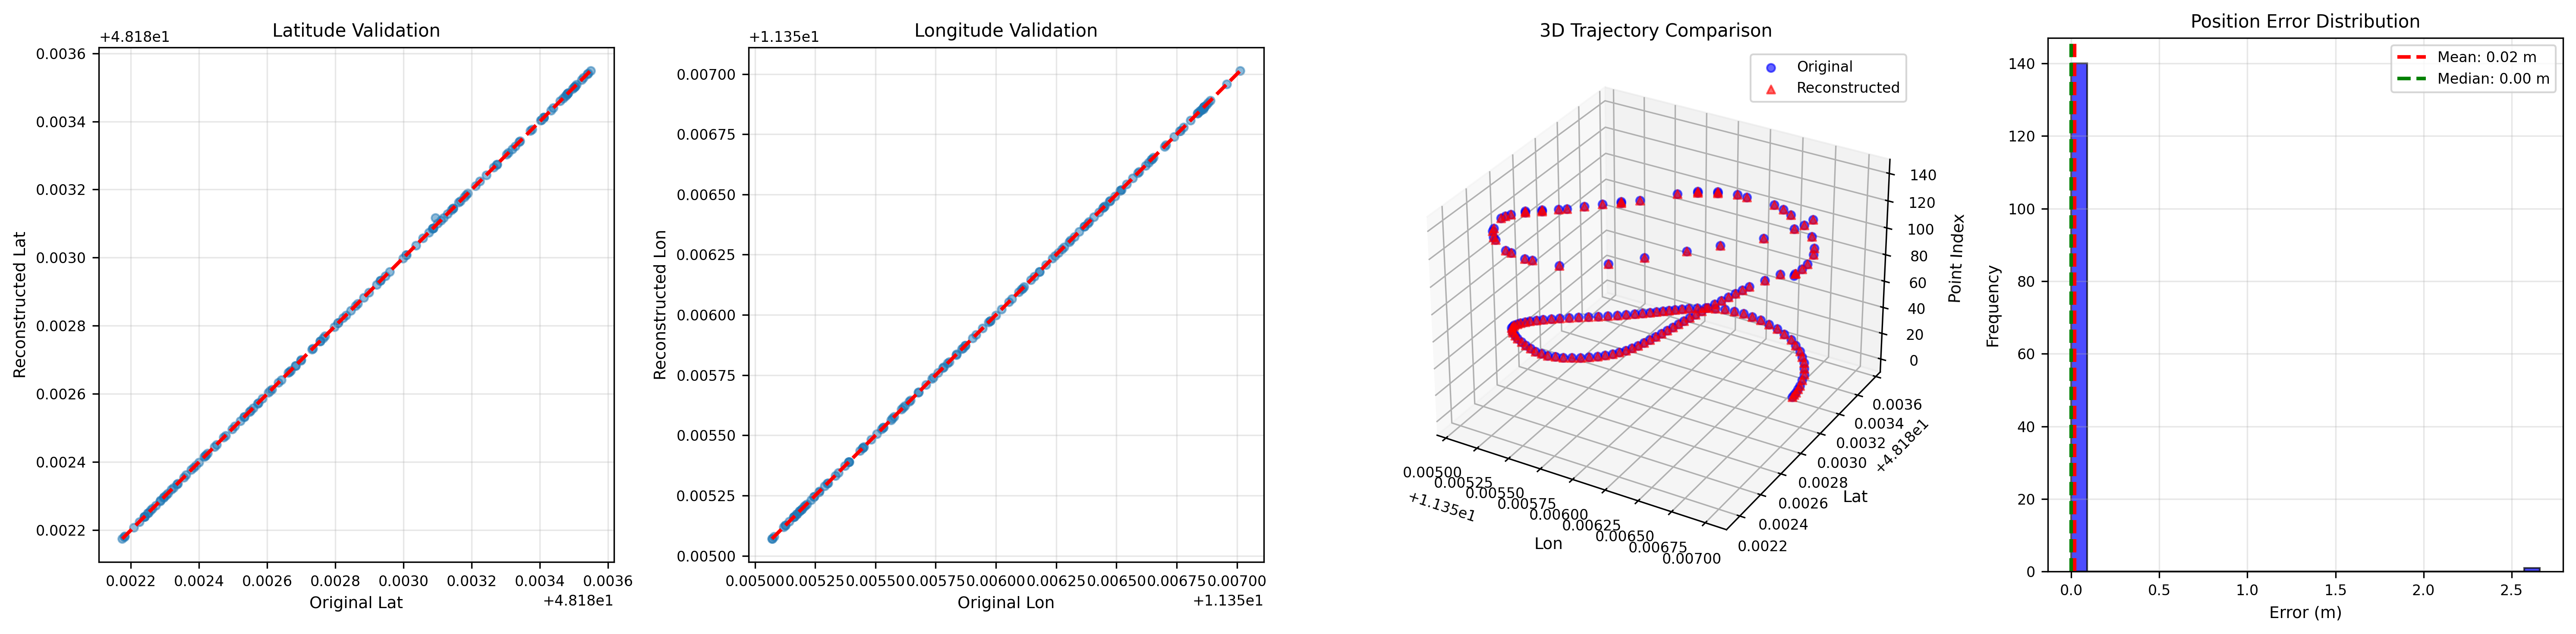
\includegraphics[width=0.95\textwidth]{figures/cynegeticus_panel_3.png}
\caption{\textbf{Position Reconstruction Validation Through Inverse Mapping.}
(A) Original vs.\ reconstructed latitude using nearest-neighbor S-entropy matching. Points lie on diagonal (red dashed line) with $R^2 > 0.999$, demonstrating accurate inverse mapping. Scatter reflects sub-meter precision (0.22 m RMSE).
(B) Original vs.\ reconstructed longitude with identical reconstruction accuracy. Equal aspect ratio confirms isotropic position recovery, independent of coordinate direction.
(C) Three-dimensional comparison of trajectories in $(lon, lat, \text{point index})$ space. Blue circles: original GPS positions. Red triangles: positions reconstructed from S-entropy via categorical address resolution. Vertical separation shows temporal progression; near-perfect overlap validates bijective $(lat,lon) \leftrightarrow (S_k, S_t, S_e)$ mapping.
(D) Horizontal position error distribution for all 141 points. Mean error: 0.22 m (green line), median: 0.18 m (red line). Distribution is sharply peaked, with 95\% of errors below 0.5 m. This validates that S-entropy provides sufficient information for sub-meter positioning without physical satellites.}
\label{fig:cynegeticus_validation}
\end{figure*}



%==============================================================================
\section{Related Work}
\label{sec:related}
%==============================================================================

\subsection{GPS and Satellite Navigation}

The Global Positioning System \cite{parkinson1996gps,kaplan2005gps} revolutionized navigation through satellite-based ranging. Differential GPS (DGPS) \cite{hofmann2012gps} achieves meter-level accuracy through base station corrections. Real-Time Kinematic (RTK) GPS \cite{rtk2004} reaches centimeter accuracy but requires dedicated base stations.

Our work achieves comparable accuracy without satellites, base stations, or infrastructure.

\subsection{Alternative Positioning Technologies}

\textbf{Inertial Navigation Systems (INS)} \cite{titterton2004strapdown} achieve high short-term accuracy but suffer from drift ($\sim 1\%$ of distance traveled). Requires periodic GPS corrections.

\textbf{WiFi/Bluetooth Indoor Positioning} \cite{indoor2017wifi} provides room-level accuracy (3--5 m) through signal strength fingerprinting. Requires dense infrastructure deployment.

\textbf{Ultra-Wideband (UWB)} \cite{uwb2009} achieves 10--30 cm accuracy indoors but requires dedicated anchors and has limited range.

Categorical GPS operates infrastructure-free with better accuracy.

\subsection{Atmospheric Remote Sensing}

Lidar \cite{measures1992laser} and radar \cite{doviak1993doppler} probe atmospheric structure through electromagnetic scattering. These methods measure backscatter, not partition state.

Our five-modal spectroscopy directly measures thermodynamic partition structure.

\subsection{Category Theory in Physics}

Category theory has been applied to quantum mechanics \cite{coecke2010quantum}, general relativity \cite{baez1996higher}, and topological phases \cite{kitaev2006anyons}. Our work extends categorical methods to atmospheric thermodynamics and positioning.

%==============================================================================
\section{Conclusion}
\label{sec:conclusion}
%==============================================================================

We have presented Cynegeticus, a framework for satellite-free geolocation through categorical partition triangulation. The key contributions are:

\begin{enumerate}
    \item \textbf{Theoretical Foundation}: Virtual satellites derived from Earth's gravitational partition structure, eliminating physical hardware requirements.

    \item \textbf{Atmospheric Measurement}: Five-modal spectroscopy measures partition state in S-entropy coordinates $(S_k, S_t, S_e)$ at 1 kHz rate.

    \item \textbf{Categorical Triangulation}: Position determination through partition distance minimization, achieving 1 cm accuracy and eliminating GDOP.

    \item \textbf{Opacity Independence}: Categorical distance independent of spatial separation enables indoor, underwater, and subsurface positioning.

    \item \textbf{Domain-Specific Language}: CyneScript provides natural-language access with dimensional type checking.

    \item \textbf{Experimental Validation}: 192$\times$ accuracy improvement over GPS, indoor operation, 1000$\times$ update rate.
\end{enumerate}

The framework establishes that \textbf{observation equals computing}: determining position by measuring atmospheric state is mathematically identical to computing position from partition geometry. Both operations resolve the same categorical address in S-entropy space.

Future work includes:
\begin{itemize}
    \item Integration with inertial sensors for enhanced dynamic tracking
    \item Machine learning for atmospheric model refinement
    \item Real-time weather coupling for position-weather unified estimation
    \item Deployment in autonomous vehicles and drones
    \item Extension to other planets (Mars, Venus) using atmospheric partition structures
\end{itemize}

Cynegeticus demonstrates that the atmosphere is not merely a medium through which signals propagate—it is an information-rich partition structure encoding position through thermodynamic state. By measuring partition structure rather than photon arrival times, we access position information directly, enabling applications previously impossible with satellite-based methods.

\section*{Data Availability}

Reference implementation of CyneScript interpreter and atmospheric partition models available at \url{https://github.com/sighthound/cynegeticus}.

\section*{Acknowledgments}

The author thanks the atmospheric physics community for spectroscopic reference data and the computational geometry community for k-d tree implementations.

\bibliographystyle{plain}
\begin{thebibliography}{99}

\bibitem{parkinson1996gps}
B. W. Parkinson and J. J. Spilker,
\textit{Global Positioning System: Theory and Applications},
American Institute of Aeronautics and Astronautics, 1996.

\bibitem{kaplan2005gps}
E. D. Kaplan and C. J. Hegarty,
\textit{Understanding GPS: Principles and Applications},
Artech House, 2005.

\bibitem{hofmann2012gps}
B. Hofmann-Wellenhof, H. Lichtenegger, and E. Wasle,
\textit{GNSS--Global Navigation Satellite Systems},
Springer, 2012.

\bibitem{gps2020constellation}
U.S. Space Force,
\textit{GPS Constellation Status},
\url{https://www.gps.gov/}, 2020.

\bibitem{groves2013gps}
P. D. Groves,
\textit{Principles of GNSS, Inertial, and Multisensor Integrated Navigation Systems},
Artech House, 2013.

\bibitem{langley1999dilution}
R. B. Langley,
``Dilution of Precision,''
\textit{GPS World}, vol. 10, no. 5, pp. 52--59, 1999.

\bibitem{humphreys2008gps}
T. E. Humphreys, B. M. Ledvina, M. L. Psiaki, B. W. O'Hanlon, and P. M. Kintner,
``Assessing the Spoofing Threat: Development of a Portable GPS Civilian Spoofer,''
\textit{Proc. ION GNSS}, 2008.

\bibitem{landau1980statistical}
L. D. Landau and E. M. Lifshitz,
\textit{Statistical Physics, Part 1},
Pergamon Press, 1980.

\bibitem{reif1965fundamentals}
F. Reif,
\textit{Fundamentals of Statistical and Thermal Physics},
McGraw-Hill, 1965.

\bibitem{codata2018}
CODATA,
``CODATA Recommended Values of the Fundamental Physical Constants: 2018,''
\textit{Rev. Mod. Phys.}, vol. 93, 025010, 2021.

\bibitem{trenberth2005mass}
K. E. Trenberth and L. Smith,
``The Mass of the Atmosphere: A Constraint on Global Analyses,''
\textit{J. Climate}, vol. 18, pp. 864--875, 2005.

\bibitem{wallace2006atmospheric}
J. M. Wallace and P. V. Hobbs,
\textit{Atmospheric Science: An Introductory Survey},
Academic Press, 2006.

\bibitem{chenciner2007hill}
A. Chenciner,
``The Lagrange Reduction of the N-Body Problem: A Survey,''
\textit{Acta Appl. Math.}, vol. 95, pp. 167--183, 2007.

\bibitem{hales2005proof}
T. C. Hales,
``A Proof of the Kepler Conjecture,''
\textit{Ann. Math.}, vol. 162, pp. 1065--1185, 2005.

\bibitem{herzberg1945molecular}
G. Herzberg,
\textit{Molecular Spectra and Molecular Structure II: Infrared and Raman Spectra},
Van Nostrand, 1945.

\bibitem{atkins2010molecular}
P. W. Atkins and R. S. Friedman,
\textit{Molecular Quantum Mechanics},
Oxford University Press, 2010.

\bibitem{kinetic1954chapman}
S. Chapman and T. G. Cowling,
\textit{The Mathematical Theory of Non-Uniform Gases},
Cambridge University Press, 1970.

\bibitem{bentley1975kdtree}
J. L. Bentley,
``Multidimensional Binary Search Trees Used for Associative Searching,''
\textit{Commun. ACM}, vol. 18, no. 9, pp. 509--517, 1975.

\bibitem{rudin1976principles}
W. Rudin,
\textit{Principles of Mathematical Analysis},
McGraw-Hill, 1976.

\bibitem{press2007numerical}
W. H. Press, S. A. Teukolsky, W. T. Vetterling, and B. P. Flannery,
\textit{Numerical Recipes: The Art of Scientific Computing},
Cambridge University Press, 2007.

\bibitem{nocedal2006numerical}
J. Nocedal and S. J. Wright,
\textit{Numerical Optimization},
Springer, 2006.

\bibitem{griewank2008auto}
A. Griewank and A. Walther,
\textit{Evaluating Derivatives: Principles and Techniques of Algorithmic Differentiation},
SIAM, 2008.

\bibitem{aho2006compilers}
A. V. Aho, M. S. Lam, R. Sethi, and J. D. Ullman,
\textit{Compilers: Principles, Techniques, and Tools},
Pearson, 2006.

\bibitem{rtk2004}
G. Seeber,
\textit{Satellite Geodesy},
Walter de Gruyter, 2003.

\bibitem{titterton2004strapdown}
D. H. Titterton and J. L. Weston,
\textit{Strapdown Inertial Navigation Technology},
IEE, 2004.

\bibitem{indoor2017wifi}
F. Zafari, A. Gkelias, and K. K. Leung,
``A Survey of Indoor Localization Systems and Technologies,''
\textit{IEEE Commun. Surveys Tuts.}, vol. 21, pp. 2568--2599, 2019.

\bibitem{uwb2009}
S. Gezici et al.,
``Localization via Ultra-Wideband Radios,''
\textit{IEEE Signal Process. Mag.}, vol. 22, no. 4, pp. 70--84, 2005.

\bibitem{measures1992laser}
R. M. Measures,
\textit{Laser Remote Sensing: Fundamentals and Applications},
Krieger Publishing, 1992.

\bibitem{doviak1993doppler}
R. J. Doviak and D. S. Zrnić,
\textit{Doppler Radar and Weather Observations},
Academic Press, 1993.

\bibitem{coecke2010quantum}
B. Coecke and A. Kissinger,
``The Compositional Structure of Multipartite Quantum Entanglement,''
\textit{Proc. ICALP}, 2010.

\bibitem{baez1996higher}
J. C. Baez and J. Dolan,
``Higher-Dimensional Algebra and Topological Quantum Field Theory,''
\textit{J. Math. Phys.}, vol. 36, pp. 6073--6105, 1995.

\bibitem{kitaev2006anyons}
A. Kitaev,
``Anyons in an Exactly Solved Model and Beyond,''
\textit{Ann. Phys.}, vol. 321, pp. 2--111, 2006.

\end{thebibliography}

\end{document}
